\subsection*{Background}
\begin{frame}{Background}
\begin{itemize}

\item Clean Air Act
\begin{itemize}
\item California violates it
\item China to blame?
\end{itemize}
\item Measure pollutants on land, near California coast
\item Compare with satellite measurements
\item informative picture - LA smog
\end{itemize}
\end{frame}
%--------------------------------------------------------------------------------------------------------------
\subsection*{Background}
\begin{frame}{PM and AOD}
\begin{itemize}

\item PM$_{2.5}$ is a particulate matter that is less than $2.5$ micrometers in diameter.

\begin{figure}[H]
\centering
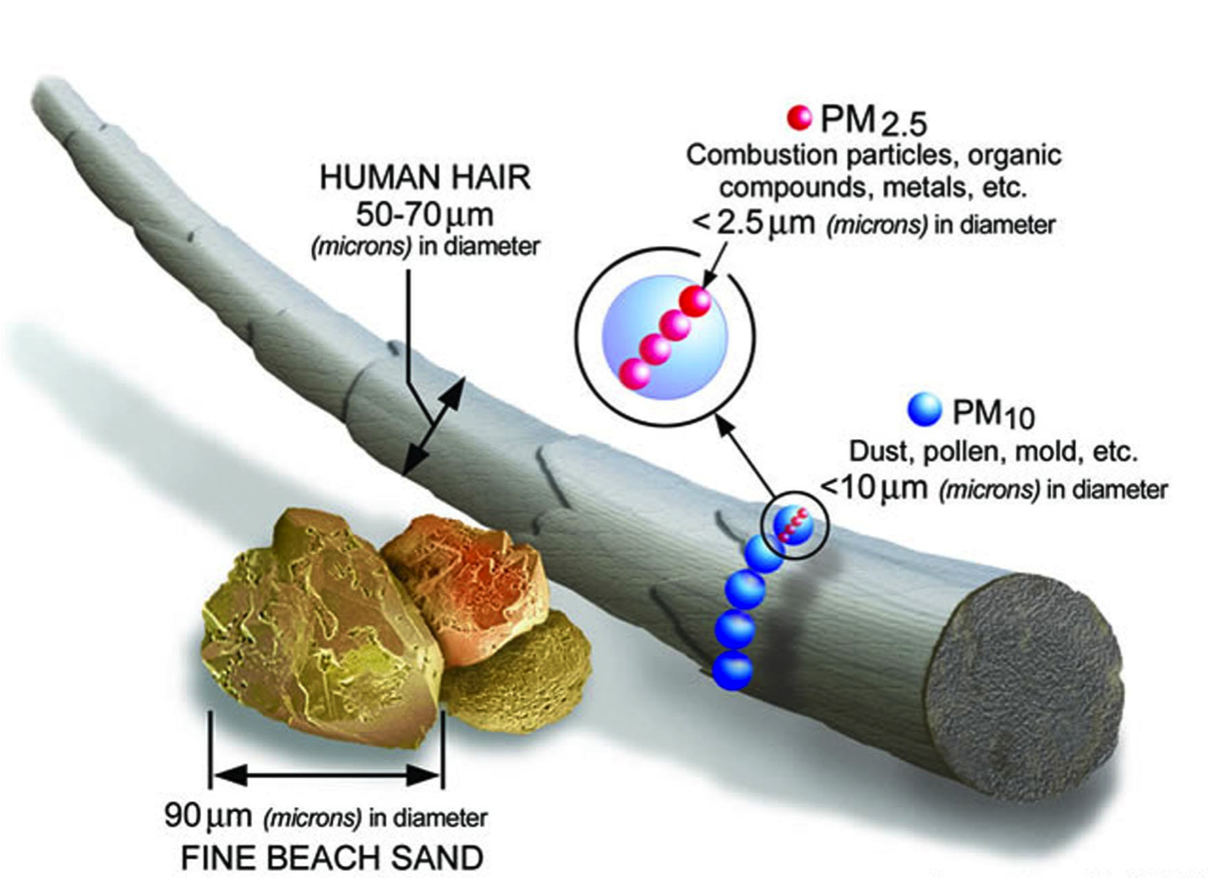
\includegraphics[scale=0.35]{hair.png}
\caption{Size of PM$_{2.5}$ compared to other particulate matter}
\label{fig:locations}
\end{figure}


\item Aerosol Optical Depth (AOD) measures the amount of light from the sun blocked by dust and pollutants.

\end{itemize}
\end{frame}

